\documentclass[11pt]{report}
%\usepackage[german]{babel}

%Graphs

\usepackage{pgfplots}
\pgfplotsset{width=15cm,height=7.5cm,compat=1.9}
\usepgfplotslibrary{external}
\tikzexternalize

%Definitions
\usepackage{amsthm}
\usepackage{mdframed}

\NewDocumentCommand\newmdtheoremenvnonumber{O{} m m }{%
  \newtheorem*{#2}{#3}
  \BeforeBeginEnvironment{#2}{%
     \begin{mdframed}[#1]}%
  \AfterEndEnvironment{#2}{%
     \end{mdframed}}%
}

\newmdtheoremenvnonumber{mydefinner}{\mydeflabel}
\newcommand{\mydeflabel}{}
\newenvironment{mydef}[1]
 {\renewcommand\mydeflabel{#1}\begin{mydefinner}}
 {\end{mydefinner}}

\newcommand{\attribution}[1]{\textup{(#1)}}



%Citations
\usepackage[style=authoryear, backend=bibtex, urldate=long, sorting=none, defernumbers=true,autocite=superscript]{biblatex}
\addbibresource{refs.bib}
\usepackage{csquotes}


%Math Library
\usepackage{amsmath}

%Images Library
\usepackage{float}
\usepackage{graphicx}
\graphicspath{ {./images/} }

%General Layout
\usepackage{geometry}
\geometry{
    a4paper,
    left=20mm,
    right=20mm,
    top=20mm,
    bottom=20mm
}


%Background image
\usepackage[pages=some]{background}

%Liks of TOC
\usepackage{color}   %May be necessary if you want to color links
\usepackage{hyperref}
\usepackage{lstmisc}

\hypersetup{
    colorlinks,
    linkcolor={blue!50!black},
    citecolor={blue!50!black},
    urlcolor={blue!80!black}
}


\backgroundsetup{
scale=1,
color=black,
opacity=1,
angle=0,
contents={%
\hspace*{13.5cm}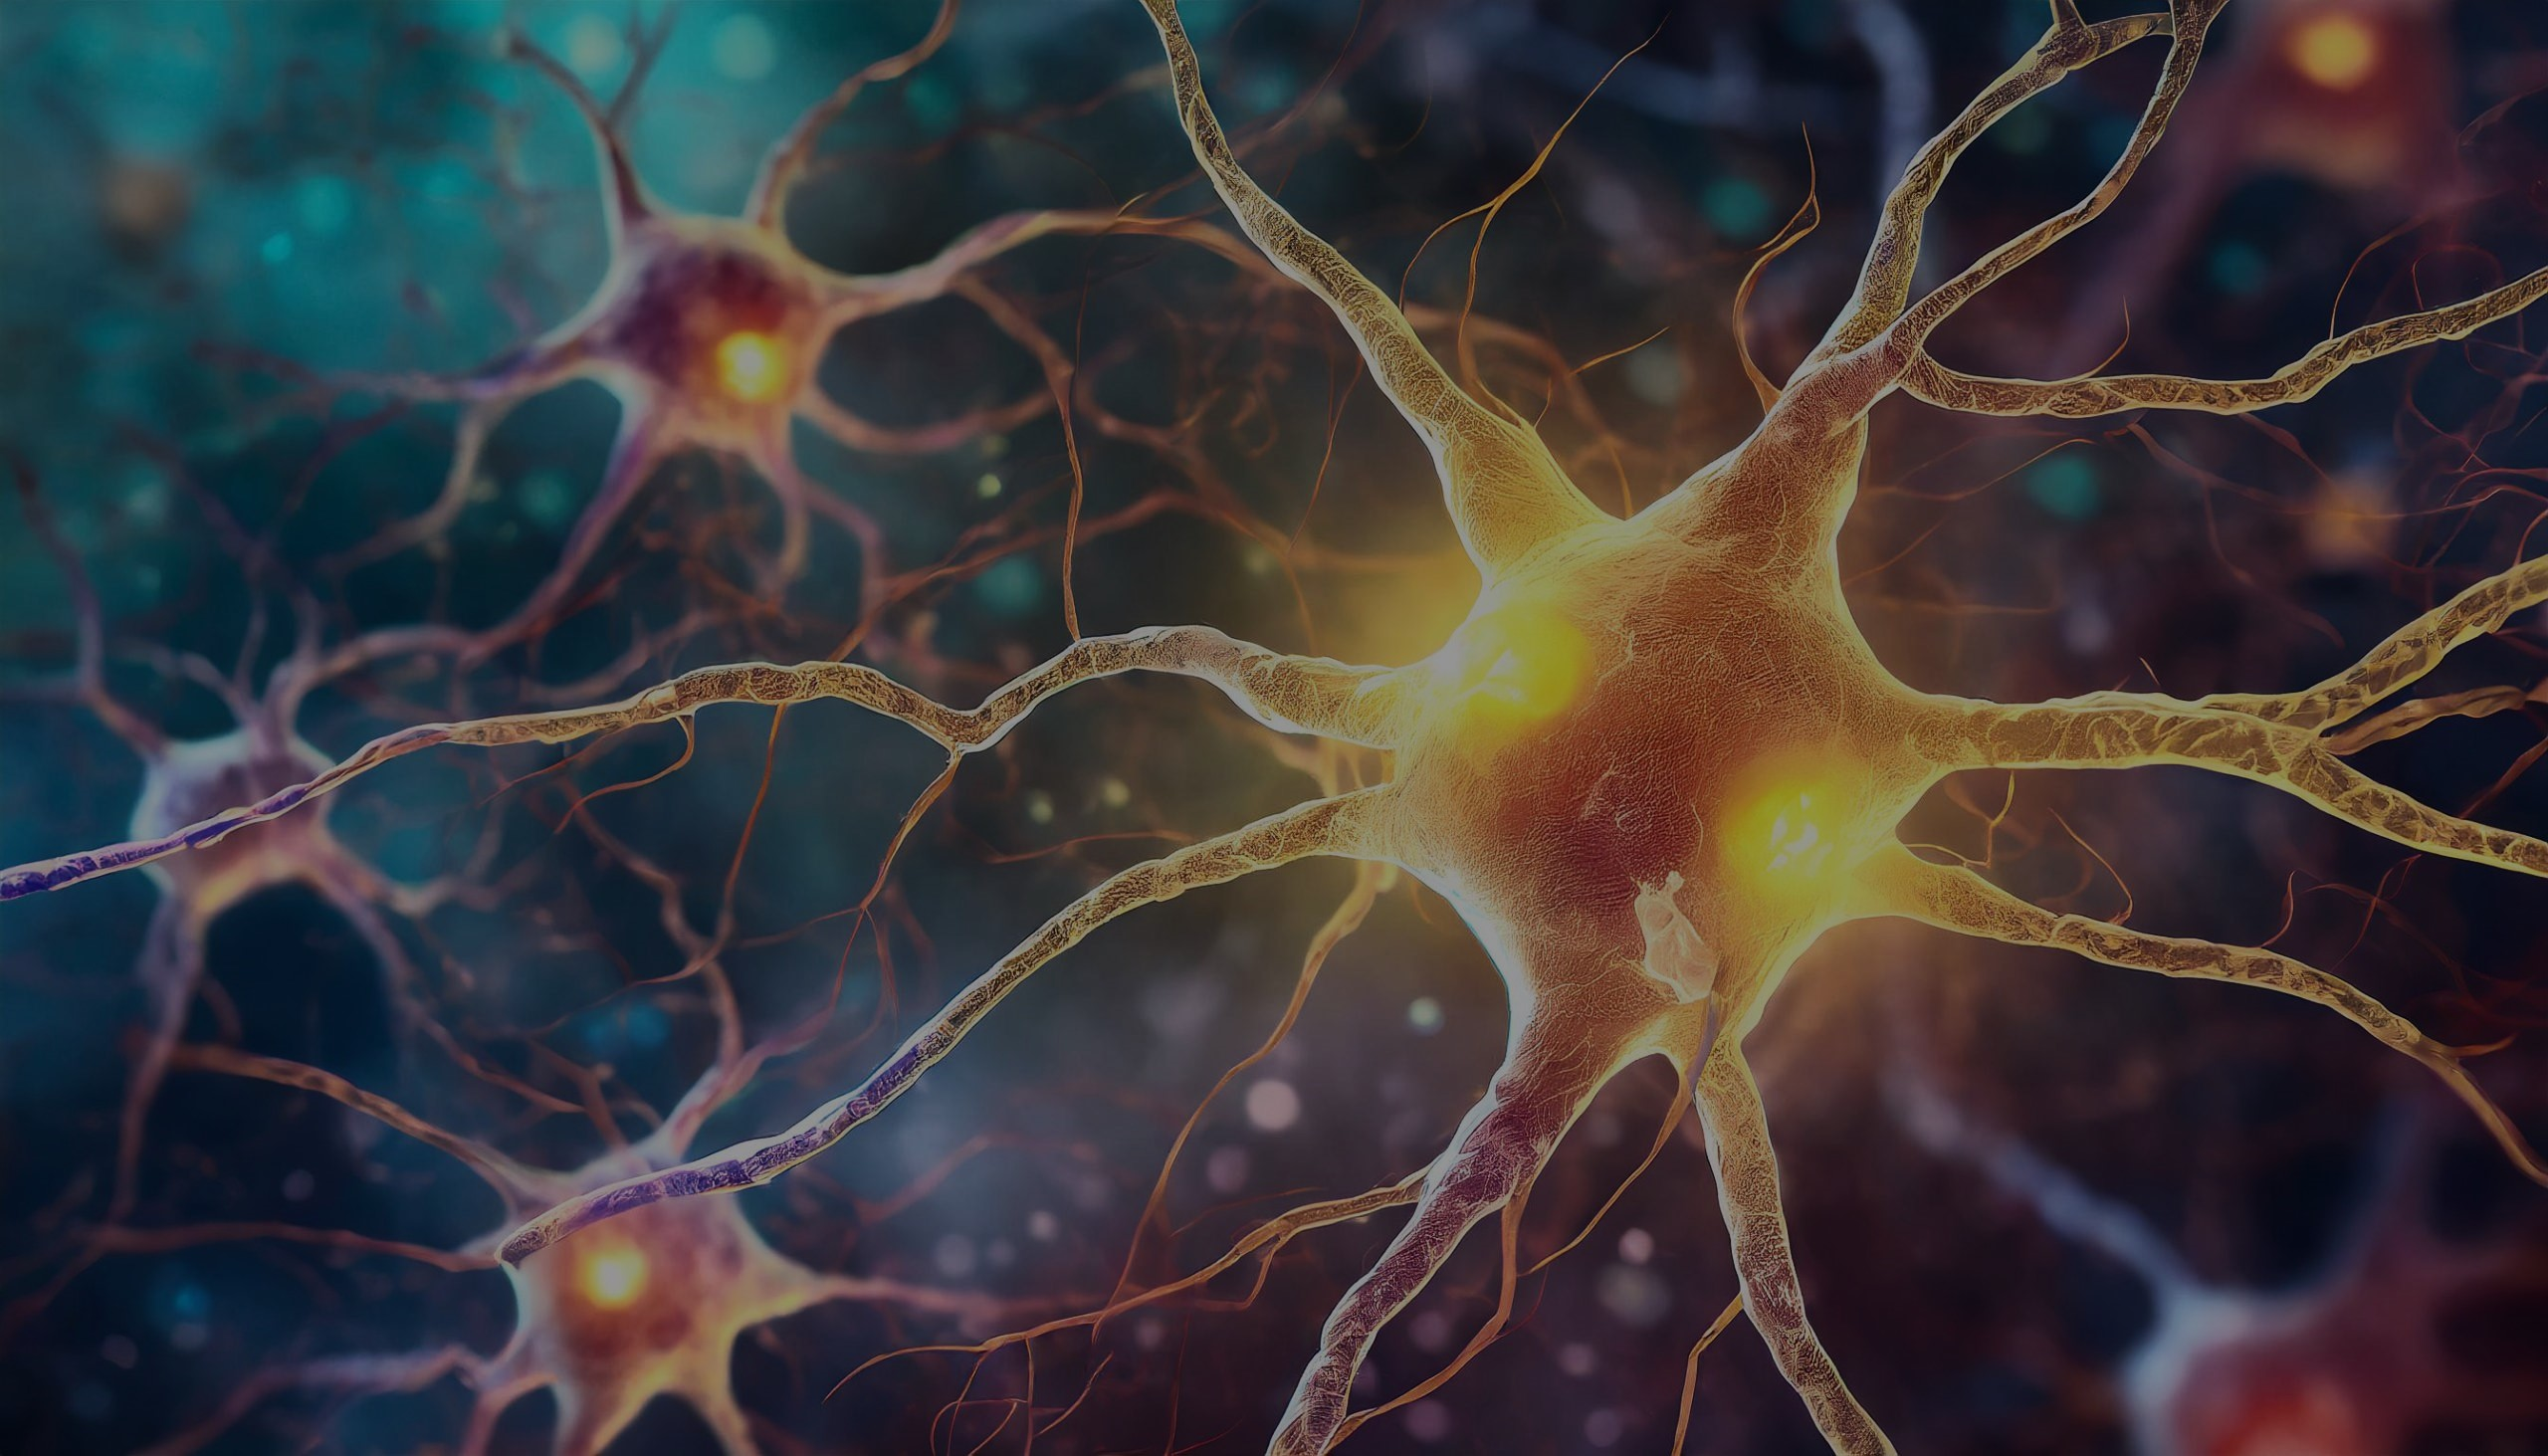
\includegraphics[width=3\paperwidth,height=\paperheight]{abstract_neurons3}
  }%
}


\begin{document}
    \pagenumbering{gobble}
    \begin{titlepage}
        \BgThispage
            \color{white} {
                \begin{center}
                    \Large \textsc{Matura Thesis}\\Kantonsschule Hohe Promenade\\
                    \rule[0.1cm]{15.8cm}{0.1mm}\\
                    \vspace{3cm}
                    \Huge \textbf{ \textsc{How can you develop \\Evolutionary Neural Networks which \\learn to play Board Games?}}\\
                    \vspace{0.8cm}
                    \Large \textit {Implementation and Study of\\ Evolutionary Neural Networks inspired\\ by the NEAT Algorithm}\\
                \end{center}
                \vspace{3cm}
                \rule[0.1cm]{15.8cm}{0.1mm}\\
                \vspace{7cm}\\
                \begin{minipage}[t]{0.47\textwidth}
                \large\textbf {Thesis By:}\\
                \end{minipage}
                \hfill
                \begin{minipage}[t]{0.47\textwidth}\raggedleft
                \large\textbf {Lucien Kissling 6e}\\
                \end{minipage}
                \begin{minipage}[t]{0.47\textwidth}
                \large \textbf {Year:}\\
                \end{minipage}
                \hfill
                \begin{minipage}[t]{0.47\textwidth}\raggedleft
                \large \textbf {2025}\\
                \end{minipage}
                \begin{minipage}[t]{0.47\textwidth}
                \large \textbf {Supervisor:}\\
                \end{minipage}
                \hfill
                \begin{minipage}[t]{0.47\textwidth}\raggedleft
                \large \textbf {Timo Schenk}\\
                \end{minipage}
                \begin{minipage}[t]{0.47\textwidth}
                \large \textbf {Co Examiner:}\\
                \end{minipage}
                \hfill
                \begin{minipage}[t]{0.47\textwidth}\raggedleft
                \large \textbf {Dr. Arno Liegmann}\\
                \end{minipage}
                \vfill
            }
        \clearpage
    \end{titlepage}
    \pagenumbering{arabic}
    \setcounter{page}{2}
    \tableofcontents
    \chapter{Introduction}\label{ch:introduction}
    \section{Preface}\label{sec:preface}
    Ever since I got into Computer Science a few years ago, I was fascinated by the Idea of Algorithms that solved various Problems.
    Therefore, I participated in the SOI (Swiss Olympiad in Informatics) where we were taught everything about developing and programming Algorithms and their Data Structures.
    \\ \\
    In recent years although, a new field of Computer Science has gained a lot of attention, where those Algorithms are not programmed by humans, but evolved by a computer.
    This field called Machine Learning immediately got my excitement and two years ago a friend of mine and I had our first practical experience with it.
    We developed a simple Neural Network, which helped us predict the color of a lego brick in front of a color sensor based on the RGB values in various lighting conditions.
    \\ \\
    A Neural Network (NN) forms the basis of most Machine Learning Models and I will therefore explain it in much detail in the following Chapters.
    In simple terms, a NN is a strongly simplified artificial model of the human brain as a NN consists of an interconnected web of Neurons through which information flows and gets computed.
    \\ \\
    Although the NN we developed two years ago already learned on its self, we still had to provide data for it to learn from.
    This meant that we had to manually scan the RGB values of the lego bricks and then label them with the color they represented.
    The aim of my Matura Thesis therefore is to take the idea of self learning a step further by developing Neural Networks, which don't need this kind of data with solutions predefined by humans.

        \section{Thesis Statement}\label{sec:thesis-statement}
    As mentioned in the previous Section, this Thesis will explore the field of Neural Networks (NNs) that learn without data provided by humans, which is called unsupervised learning.
    The solution this Thesis will focus on are Evolutionary Neural Networks (ENNs), a combination of Neural Networks and Genetic Algorithms.
    \\ \\
    In this Thesis, I develop my own simplified implementation ENNs and then train them on Board Games to see how well it can learn to play them using different Parameters and Features.
    My approach draws inspiration from the NEAT Algorithm developed by Kenneth O. Stanley and Risto Miikkulainen in 2002, where the NNs start minimally in the first generation and then develop complexity over time.\footcite[p.105-106]{Neat_02}
    The first game I will train the ENNs on is Nim, a simple game where two players take turns removing matches from different stacks.
    \\ \\
    In specific, this Thesis aims to answer following questions:
    \begin{itemize}
        \item How can you develop Evolutionary Neural Networks (ENNs) that learn to play Board Games?
        \item How do different parameters and features of ENNs affect the learning process?
        \item How does this Implementation of ENNs compare to other Machine Learning Algorithms?
    \end{itemize}
    \chapter{Background}\label{ch:background}
    \section{Neural Networks (NNs)}\label{sec:neural-networks-(nns)}
    As already touched on in the Preface(\ref{sec:preface}), an artificial neural network (ANN or NN) is a mathematical model for data processing, initially inspired by the structure of the brain\footcite{Chandra_22}.
    Therefore, we will first have a brief look at the functioning of a brain.
            \subsection{Neurons in the Brain}\label{subsec:neurons-in-the-brain}
    Inside the brain, around 86 million neurons\footcite{caruso_23} form connections to each other through which they activate other neurons.
    In a neuron, the signals of connected neurons add up and when they reach a certain threshold, the neuron is activated and fires a signal to its own connections\footcite{Newman_23}.
    The neuron then resets after a certain amount of cooldown time.
    With this web of neurons inside the brain, animals can process information from nerve signals from the body and output them again as nerve signals instructing the body.
            \subsection{Feed Forward Neural Networks (FNNs)}\label{subsec:feed-forward-neural-networks-(fnns)}
    Now how do we apply those ideas about Neural Networks learned from the biology of a brain to a program that runs on a computer?
    The first step is to simplify the chaos of neurons in the brain into layers of neurons.
    We get an input layer, an output layer and optional so-called hidden layers in between.
    As a next step, in each layer, we connect its neurons to neurons of following layers, typically exclusively to neurons of the next layer.
    \\
    Now, the structure of our network looks something like this:
    \begin{figure}[H]
        \centering
        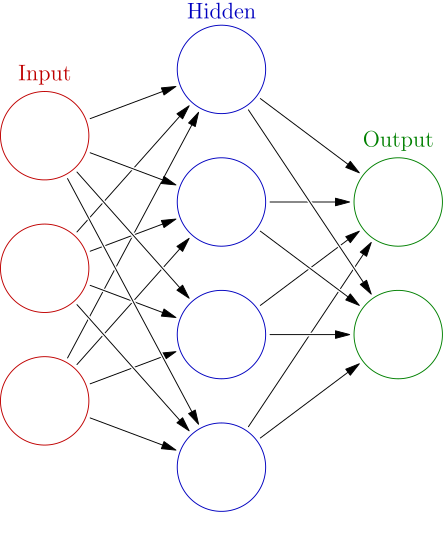
\includegraphics[width=0.25\textwidth]{nn_simple_1}~\caption{A simple Feed Forward Neural Network (FNN) with three layers: Input, Hidden and Output.\footnote{\cite{nn_simple_img_1}}}
        \label{fig:nn_simple_1}
    \end{figure}
    \noindent
    The Structure of a NN is also called Topology.
    \begin{mydef}{Neural Network Topology}
        The Topology of a Neural Network is its distinct arrangement of neurons, layers and the connections between the neurons.
        \label{definition:Topology}
    \end{mydef}
    \noindent
    For the neural network to perform functions, we also need to assign a weight to all the connections.
    This weight value ranges from -1 to 1 and can be thought of as the strength of a connection between neurons.
    \\
    In terms of computer science, this structure now resembles a directed, weighted graph, which is why we will call the neurons nodes and their connections edges from now on.
    \\ \\
    Now let's see, how information gets computed by a neural network by using the example of a computer vision NN, that recognizes digits on a black/white image:
    First, we need a way to encode the information into values for the nodes of the input layer, in our example the Brightness values of the single pixels.
    We assign these values to the nodes of the input layer.
    \\
    Then, for each node of the input layer, we look for all edges connected to that node.
    For each of these edges we multiply its weight by the value of the input node and add the result to the other node connected by the edge.
    \\
    After iterating through all the nodes of the one layer, we move the next layer.
    Now, the value of the nodes in this layer is the sum accumulated by the value of all connected nodes multiplied the weight of that connection:
    \begin{equation}
        v_x = \sum_{i=0}^{N}v_i * w_i\label{eq:sum_connected_nodes}
    \end{equation}
    Where:
    \textit{
        \begin{itemize}
            \item N is the number of connected nodes
            \item $v_x$ is the value of the current node
            \item $v_i$ is the value of the current node
            \item $w_i$ is the weight of the edge connecting the current node to node i
        \end{itemize}
    }
    \noindent
    Additionally, we can add a bias value $r_x$ ranging from -1 to 1 onto the value of the nodes.
    Afterward, an activation function is applied to the value of the nodes to fit the value of the node inside a preferred range.
    This activation function can also be thought of as the threshold of stimulation for a neuron to fire.
    Two examples for activation functions are:
    \begin{itemize}
        \item Sigmoid Function: $\sigma(x) = \frac{1}{1 + e^{-x}}$
        \item Rectified Linear Unit (ReLU): $\sigma(x) = \max{0, x}$
    \end{itemize}
    Plot of the activation functions:
    \\ \\
    \begin{center}
    \begin{tikzpicture}
     \begin{axis}[
     xmin=-6,
     xmax=6,
     ymin=0,
     ymax=6,
     ytick distance = 1,
     xtick distance = 1,
     minor tick num=1,
    axis lines = left,
    line width = 1.5pt,
    grid=both,
    major grid style={line width=0.8pt,draw=gray!50},
    minor grid style={line width=0.4pt,draw=gray!20},
    xlabel = \(x\),
    ylabel = {\(\sigma(x)\)}]
     \addplot[
        domain=-10:10,
        color=red,
        samples=1000.,
     ]{1/(1 + e^-x)};
\addlegendentry{\(Sigmoid\)}
     \addplot[
         domain=-10:10,
         color=blue,
         samples=1000.,
     ]{max(0,x)};
     \addlegendentry{\(ReLU\)}
     \end{axis}
    \end{tikzpicture}
    \end{center}
    \\ \\
    The final function for the value of one node is therefore:
    \begin{equation}
        v_x = \sigma\left(\sum_{i=0}^{N}v_i * w_i + r_x\right)\label{eq:value_node}
    \end{equation}
    Where (additionally to equation~\ref{eq:sum_connected_nodes}):
    \textit{
        \begin{itemize}
            \item $r_x$ is the bias of the node
            \item $\sigma$ is the activation function
        \end{itemize}
    }
    \noindent
    Now this value $v_x$ can be used in upcoming layers.
    When we reach the final layer after iterating through all the nodes and layers of the NN, we can read out its computed output.
    This output again is encoded in node values like the input and therefore needs to be decoded for the result.
    In the example of a digit detecting NN, we could encode the output with 10 output nodes, each representing one digit.
    The result could be decoded by using the output node with the highest value as result.
    This kind of output encoding, where all possible result get their own node is called One-hot encoding.
    With this kind of output encoding, the values of the output nodes can be interpreted as a certainty value for a specific result to be correct.
            \subsection{Remark: Functioning of NNs}\label{subsec:remark-about-the-funtioning-of-nns}
    Now that we have established how a NN works, it is important to understand why this kind of algorithm is revolutionary to computer science.
    \\ \\
    An algorithm is a set of functions applied in a certain order onto an input to receive a result.
    Traditionally, this algorithm was programmed with the help of mathematical operations, logic functions, loops, system functions and data structures, which are then converted into binary code for the processor.
    Of course, this also applies in the context of NNs, however, there is also a third layer of abstraction on top, which simulates the functioning of a brain with neurons.
    Since the traditional algorithm only enables the neurons in the NN, the third neuron-based layer is what computes the actual function of the NN\@.
    Therefore, NNs resemble more the functioning of a brain than a traditional algorithm.
    This difference results in implications for the functioning of an NN:
    Traditional algorithms represent actual mathematical calculations and are therefore deterministic.
    With NNs, the algorithm is based on different parameters for nodes and edges, which make it an unpredictable blackbox.
    Additionally, NNs don't represent actual functions but try to approximate them instead.
    This means it is hard to prove a neural network to be always accurate and is the reason why we often call the result of NNs its prediction.
            \subsection{An Example of NN learning: Backpropagation}\label{subsec:an-example-of-nn-learning:-backpropagation}
    We already know how a NN can make a prediction for a given input with the help of parameters, which encode for the structure and weights/biases of the NN.\@
    But how do we find such parameters for a given problem?
    The answer is to use machine learning, which trains the model to perform a certain task with the help of training data.
    \begin{mydef}{Machine Learning}
        Machine Learning is a subset of artificial intelligence that involves the use of algorithms and statistical techniques to optimize artificially intelligent models for a given problem.
    \end{mydef}
    One machine learning algorithm for NNs is called backpropagation, which is one of the simplest and most efficient ways to train a NN.\@
    \begin{mydef}{Backpropagation}
        The backpropagation algorithm is an algorithm that can optimize parameters for weights and biases of a NN within a fixed topology for a certain problem with the help of labeled data.
    \end{mydef}
    Backpropagation uses a training and test set containing unlabeled data for a problem.
    But what does a test set with unlabeled data mean in the context of machine learning?
    \begin{mydef}{(Un)labeled Data}
        Labeled data for a machine learning problem is a set of data with sample problems and the respective solutions.
        Unlabeled data instead only contains the sample problems.
    \end{mydef}
    The Machine Learning Process starts with an NN with fixed topology and random weights/biases.
    Then, you give the NN the training problems, whose predictions will be random at first.
    However, with the help of the corresponding solutions, you can refine the predictions of the NN by adjusting the parameters in a way that would let the NN make the correct prediction for the given problem.
    This is done by starting from the prediction of a certain problem its solution and propagating back through the whole NN until reaching the input layer.
    More specifically, you compute a cost function of
    The NN shouldn't be adapted only to a single problem but should be able to make accurate predictions for the whole training set as well as for unknown problems.
    To therefore prevent overcorrecting a NN for a single problem, we have to factor in a learning rate significantly smaller than 1 onto our correction.
    No we can train the NN on the whole training set for many generations, until the NN starts to make accurate predictions for the whole.
    To test the performance on unknown problems we can use a separate test set, which the NN wasn't trained on.

        \section{Evolutionary Computation (EC) \& Genetic Algorithms (GAs)}\label{sec:evolutionary-computation-(ec)-&-genetic-algorithms-(gas)}
    Now we will have a look at the Machine Learning Technique, this Thesis focuses on.
    Again, we will draw inspiration from Nature:
    \begin{mydef}{Evolutionary Computation}
    Evolutionary Computation (EC) is an Algorithm that optimizes a set of parameters for a problem with the help of natural selection.
    \end{mydef}
    One scenario for EC might be for example if you have a large set of data points of an unknown polynomial function with noise and outliers.
    If you want to find the underlying polynomial function, you could then employ Evolutionary Competition to find the best fitting parameters for such polynomial.
    So how do you find these parameters?
    \\ \\
    You start with an initial population of agents with a random set of parameters.
    For each generation of your population you will then repeat following steps:
    \begin{itemize}
        \item Fitness: First, you need to find out how good each agent (and its parameters) performs in the function they try to optimize for.
        The fitness evaluation can be done with an objective cost function or a competition between the agents, which evaluates their relative performances.
        In our example, the cost function might be the sum of the absolute differences between the data points and the output of the polynomial function.
        \item Selection: As a next step, you rank the agents performances to then pick the ones that have performed the best.
        \item Reproduction: The best agents pick is the part of the population that survives.
        These agents will then be replicated by copying their parameters (asexual reproduction) of by merging parameters from different agents (sexual reproduction).
        \item Mutation: The agents parameters will then be mutated by either completely overwriting certain parameters with new random parameters or by shifting the existing parameters by a random number.
    \end{itemize}
    After a certain number of generations, you will then have the best performing set of parameters for a given problem.
    There is also one popular addition to EC, which draws inspiration from nature again:
    \begin{mydef}{Genetic Algorithm}
    A Genetic Algorithm (GA) is an implementation of EC that uses a genetic representation of the parameters.
    \end{mydef}
    Its main idea is to have genes, that only encode indirectly for the parameters, and that can be on and off.

        \section{Evolutionary Neural Networks (ENNs)}\label{sec:evolutionary-neural-networks-(enns)}
    After having covered all the basics about NNs and EC, we can now combine those concepts to create the algorithm, that this thesis is about.
    \begin{mydef}{Evolutionary Neural Networks}
        Evolutionary Neural Networks (ENNs) are Neural Networks that use Evolutionary Computation to optimize for its parameters for the NNs weights/biases and its topology.
    \end{mydef}
    ENNs are useful for complex machine learning problems and also work for unlabeled training data as long as there is a fitness function.
    Let's bring our knowledge about EC into the context of Neural Networks:
    The parameters ENNs encode for are for the weights, biases, nodes and edges of a Neural Network.
    You could either directly encode the NNs parameters as a graph or indirectly as genes, which would make it a Genetic Algorithm.
    ENNs still start with a random population of agents that are evaluated and selected by a fitness function.
    Then they replicated (sexually or asexually) and finally mutated in following ways:
    \begin{enumerate}
        \item Change weights/biases: A new random value is set for the weight or bias of a random existing edge or node.
        \item Shift weights/biases: The value for an existing weight or bias of a random existing edge or node is altered by a random change but is kept close to the old value.
        \item Add edges: A new edge is added between two random unconnected nodes.
        \item Add nodes: A new node is added in between of a random existing edge.
        The old edge is removed and two new edges with random weight are added between the new node and the two other nodes each.
        \item Remove nodes/edges: A random node or edge in a way that doesn't cut off the input from the output layer.
    \end{{enumerate}}
    \section{Drawing Inspiration from the NEAT-Apporach}\label{sec:drawing-inspiration-from-the-neat-apporach}
        As already stated in the Thesis Statement(\ref{sec:thesis-statement}), Neuroevolution of Augmenting Topologies is a ENN machine learning algorithm by Kenneth O. Stanley and Risto Miikkulainen in 2002\footcite[p.105-106]{Neat_02}.
        One of its main innovations is that the initial population starts with NNs of lowest complexity and only increase topological complexity as its useful for the problem.
        In specific, you start with NNs that have only the nodes of the input layer connected to the nodes of the output layer.
        This should result in more efficient NNs for the problem, as the complexity is only increased when it improves the NNs performance.
        The NEAT algorithm therefore only needs the mutations 1. to 4. showed in the last chapter(\ref{sec:evolutionary-neural-networks-(enns)}) and doesn't need to remove complexity (mutation 5.)as it is already minimal.


    \section{Related Work}
    \chapter{Building my ENN}
        \section{Basic Implementation}
            \subsection{Neural Network}
            \subsection{Mutation}
            \subsection{Natural Selection}
            \subsection{Nim}
            \subsection{Data Saving}
        \section{First Findings}
            \subsection{Simple Nim}
            \subsection{Nim}
        \section{Complexification}
    \chapter{Wrapping Up}
        \section{Auto Review}
        \section{Future Work}
    \chapter{Appendix}
        \section{Code}
        \section{Data}
        \section{Documentation}
        \section{References}
    \printbibliography

\end{document}
